% Chapter Template

\chapter{Marco Teórico} % Main chapter title

\label{Chapter2} % Change X to a consecutive number; for referencing this chapter elsewhere, use \ref{ChapterX}

%----------------------------------------------------------------------------------------
%	SECTION 1
%----------------------------------------------------------------------------------------

Hablar de ZOWI.
De los Servos.
Calibración. usual arduino-servos
Hablar de las IMUS. Principio teórico.
Placas?

%-----------------------------------
%	SUBSECTION 1
%-----------------------------------
\section{Contexto}

Una de las líneas de desarrollo de BQ es la robótica educativa, un conjunto de productos y servicios orientados a educar en las tres partes de todo proyecto tecnológico: Diseño, hardware y software. Cuenta para ello con diferentes productos (impresoras -Witbox, hephestos-, "mi primer kit de robótica", o los printbots), programas (Bitbloq -basado en scratch-), así como contenido y soporte en la web ("Do it with others" -www.diwo.bq.com-).

El presente proyecto surge de la necesidad de automatizar una parte del proceso de fabricación de un nuevo robot educativo, Zowi. Hasta ahora, los robots desarrollados (printbots, por su carácter de chasis y componentes no-electrónicos totalmente imprimibles en 3d) usaban para moverse servos y ruedas, Zowi es el primer robot bípedo desarrollado por BQ (utiliza dos servos para los piés y otros dos para las caderas) y la librería de osciladores sinusoidales -oscillator-. Desarrollada por Juan "Obijuan" González, entonces jefe del departamento, para robots serpiente modulares.

\subsection{Zowi}
Zowi, también llamado el robot de Clan TVE, es un robot educativo para niños que les inicia en el mundo de la tecnología y de la programación.

Este robot, además de los servos que lo convierten en un robot bípedo, incorpora unos sensores de ultrasonidos como ojos que le permiten detectar obstáculos, una matriz de leds como boca para expresar "emociones", 3 pequeños botones para alternar entre sus modos de funcionamiento.

Se ha creado una aplicación móvil, Zowi App, que permite controlar los movimientos de Zowi y reprogramarlo fácilmente con diferentes juegos.

Zowi tiene muchas más posibilidades más allá de lo predefinido en su aplicación. BQ tiene una plataforma online para programar a sus robots y placas de una forma muy sencilla. Esta plataforma se llama Bitbloq. En ella se puede programar a Zowi y a otros tipos de placas Arduino de forma muy sencilla por medio de bloques. Tambien se puede emplear código directamente.

\section{Motivo del proyecto}
La tarea asignada al autor del proyecto fue la de idear y desarrollar el prototipo de un sistema capaz de ajustar de forma automática cada uno de los 4 servos que componen las piernas de Zowi, lo que permite al robot ejecutar sus programas de fábrica, con los que saldrá a la venta, de forma correcta; entre ellos: realizar diferentes bailes, caminar, etc. Dicho sistema debe ser utilizado por operaradores sin conocimientos de arduino ni de electrónica en general y, en principio, se desconoce su nacionalidad (razón por la que parte de la documentación anexada se encuentra en inglés: menú de la interfaz, comentarios del código, etc).

\subsection{Servos}
Los servos son un tipo especial de motor de c.c. que se caracterizan por su capacidad para posicionarse de forma inmediata en cualquier posición dentro de su intervalo de operación. Para ello, el servomotor espera un tren de pulsos que se corresponde con el movimiento a realizar. Están generalmente formados por el motor, un sistema reductor formado por ruedas dentadas, un potenciómetro y un circuito de realimentación, todo en un misma caja de pequeñas dimensiones.
El circuito electrónico de realimentación es el encargado de recibir la señal PWM y traducirla en movimiento del Motor DC. El eje del motor DC está acoplado a un potenciómetro, el cual permite formar un divisor de voltaje. El voltaje en la salida del divisor varía en función de la posición del eje del motor DC.

La modulación por anchura de pulso, PWM (Pulse Width Modulation), es una de los sistemas más empleados para el control de servos. Este sistema consiste en generar una onda cuadrada en la que se varía el tiempo que el pulso está a nivel alto, manteniendo el mismo período, con el objetivo de modificar la posición del servo según se desee. Arduino permite generar PWM en algunos de sus pines de forma sencilla, además, para hacerlo aún más fácil, tiene la librería \textit{srvo.h}, que nos permite dar un valor de posición angular (grados) a un determinado pin, y él sólo realiza genera el PWM.

Las señales de PWM requeridas para que el circuito de control electrónico son similares para la mayoría de los modelos de servo. Esta señal tiene la forma de una onda cuadrada. Dependiendo del ancho del pulso, el motor adoptará una posición fija.

\subsection{Problema a resolver}
Los servos empleados son una versión clónica del Futaba S3003, con un rango de funcionamiento algo mayor (en torno a 187º). Para el caso de Zowi, el rango empleado será bastante menor, por cuestiones de estabilidad del juguete y por el diseño de las piezas, mecánicamente sería imposible torcer las articulaciones en todo el rango del servomotor.

La continuación del eje del servo, eje dentado (ver Figura \ref{fig:EjeServo} para referencia), engrana en la pieza de Zowi, como podemos ver en la Figura \ref{fig:EjeServo}, hay un determinado número de dientes. Para el servo empleado en Zowi, el número de dientes es 24. Un diente supone un cambio de 15º respecto al anterior. El ensamblaje se lleva haciendo que el servo llegue a hacer tope con un extremo, sin embargo, dentro de esos 15º y por fabricación del servo, las piezas tienen un desfase de hasta 7.5 grados, o mayor aún si el operador no elige bien la orientación al engranar. Adicionalmente, por el fabricante del servo, la relación del tren de pulsos PWM y la posición final del servo puede variar, incluso variar muy ligeramente entre servos del mismo fabricante. Tenemos entonces varios factores que hacen que cada servo sea montado en una posición distinta y tenga que ser configurado por software.

\begin{figure}
\centering
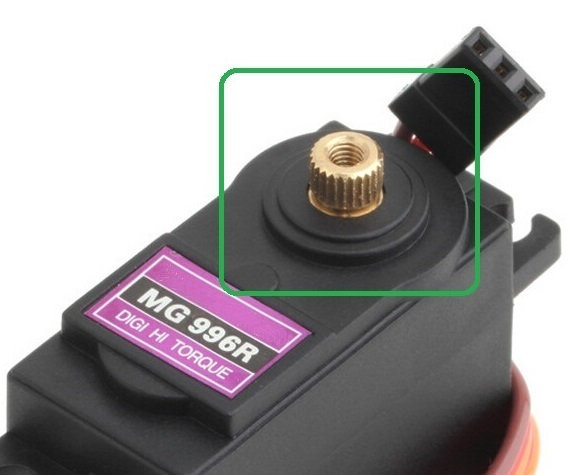
\includegraphics[width=120mm]{Figures/servo-shft.jpg}
\caption[Eje dentado servo]{Eje dentado servo}
\label{fig:EjeServo}
\end{figure}

Lo ideal sería que la posición del servo intermedia coincidiese con la posición neutra de la articulación de Zowi, dejando la mitad del rango de giro del servomotor para cada sentido. Como el rango de movimiento del juguete es mucho menor que el rango completo del servo, se tiene cierto margen para permitir su ajuste.

\subsubsection{Calibración}
La calibración de los servos es de importancia vital para un buen funcionamiento de las funciones programadas en el juguete. En arduino, utilizando la librería "srvo.h", se consigue una equivalencia entre números enteros y grados sexagesimales. El primer paso para utilizar un servo es siempre definir qué posición es la de partida del servo, ésto se realiza guardando un valor "trim" u "offset" que será el valor (positivo o negativo) que hace que el servo esté en la posición deseada como 0º.

Cuando el usuario quiere mover el servo a una posición determinada, tendrá que moverlo a la posición "deseada + offset", el offset obviamente siempre será el mismo, salvo que desmonte y monte el servo en la misma pieza en otra posición o en otras piezas. Este ajuste es habitual cuando se trabaja con servos, en robótica o radiocontrol, por ejemplo. Zowi  un producto pensado para ser reprogramado y "trasteado", para que el usuario aprenda sobre electrónica y programación, pero éste usuario no tiene por qué tener ningún conocimiento previo, es por ésto que se da con programas por defecto que muestran sus posibilidades y con los valores de "offset" de los servos para el montaje de fábrica guardados en determinadas direcciones de la EEPROM, zona de la memoria de la placa controladora que no se borra al ser reprogramada.

\section{Posibles alternativas}

Anteriormente se ha explicado cuál es el problema a resolver. Para darle solución, la clave es poder leer las orientaciones reales de los servos, es decir, respecto al mismo juguete; en base a estas posiciones actuar sobre los servos hasta colocarlos en la posición neutra y guardar el desfase observado de cada servo. Se plantean dos posibles caminos:

\begin{itemize}
  \item \textbf{Visión por computador:} Emplear un sistema de visión para, mediante matching y detección de líneas, observar el desvío y poder actuar sobre los servomotores hasta llevarlos a la posición deseada.
  \item \textbf{Visión por computador:} Utilizar utillaje impreso y sensores de tipo inercial (acelerómetro-giróscopo) para calcular las inclinaciones producidas por la posición de los servos.
\end{itemize}

Se elige la segunda opción por tener una estimación de tiempo de desarrollo más ajustada, además de un coste considerablemente menor.

\subsection{Sensor IMU}
Una IMU o unidad de medición inercial, es un sensor diseñado para combinar las características de un acelerómetro y un giróscopo y mostrar información completa sobre aceleración, posición, orientación, velocidad...

Las medidas crudas de los componentes del acelerómetro, giróscopo y magnetómetro estarán directamente relacionadas con la fuerza G, velocidad angular y campo magnético, respectivamente. Dichas medidas pueden ser procesadas y tratadas con un microcontrolador o microprocesador para obtener posiciones, orientaciones, etc.

\subsubsection{Acelerómetro}

El acelerómetro mide la aceleración en las 3 dimensiones del espacio.La gravedad de la Tierra tiene una aceleración de aproximadamente 9.8 m/s\textsuperscript{2}, perpendicular al suelo. Así pues, la IMU también detecta la aceleración de la gravedad terrestre. Gracias a ésta se pueden usar las lecturas del acelerómetro para saber cuál es el ángulo de inclinación respecto al eje X o eje Y.

\begin{figure}
\centering
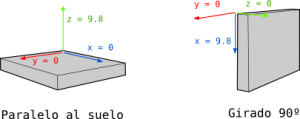
\includegraphics[width=90mm]{Figures/imu-acel.png}
\caption[Lectura acelerómetro]{Lectura acelerómetro}
\label{fig:ImuAcel}
\end{figure}

Dado que el ángulo se calcula a partir de la gravedad, no es posible calcular el ángulo Z empleando únicamente el acelerómetro. Para hacerlo se necesita otro componente: el magnetómetro, que es simplemente un tipo de brújula digital.

\subsubsection{Giróscopo}


%-----------------------------------
%	SUBSECTION 1
%-----------------------------------
\section{Herramientas y tecnologías utilizadas}
